%----------------------------PREAMBLE--------------------------------------------------
\documentclass[9pt]{beamer}
\usetheme{Malmoe}
\usecolortheme{beaver}

\usepackage{stdheader}
\usepackage[subpreambles=true]{standalone}
% Custom figs/diagrams
%\usepackage{tikz}
%\usetikzlibrary{positioning}

\DeclareMathOperator\Tr{Tr}
\graphicspath{{../figs/}}

\AtBeginSection[]
{
  \begin{frame}
    \sectionpage
    \tableofcontents[currentsection, hideothersubsections]
  \end{frame}
}

\setbeamertemplate{navigation symbols}{}

%\title{The Berry Phase}
%\author{Jacob MacWilliams}
%-----------------------------TITLE PAGE/TOC--------------------------------------------
\begin{document}

%\documentclass[beamer]{standalone}
\usetheme{Malmoe}
\usecolortheme{beaver}
\usepackage[T1]{fontenc}
\usepackage{tikz}
\usepackage{pdfrender}
\usetikzlibrary{shapes,arrows}
\title[]{The Berry Phase}
\date{29 July 2022}
\author[]{Jacob MacWilliams}
\institute[]{Universität Konstanz}
\setbeamerfont{author}{size=\Large}
\setbeamerfont{institute}{size=\fontsize{10}{10}\itshape}
\setbeamerfont{title}{size=\fontsize{30}{36}\bfseries}
\setbeamerfont{subtitle}{size=\Large\normalfont\slshape}
\setbeamertemplate{title page}{%
    \begin{tikzpicture}[remember picture,overlay]
    \node[anchor=south] at ([yshift=-0.15cm]current page.south)
      {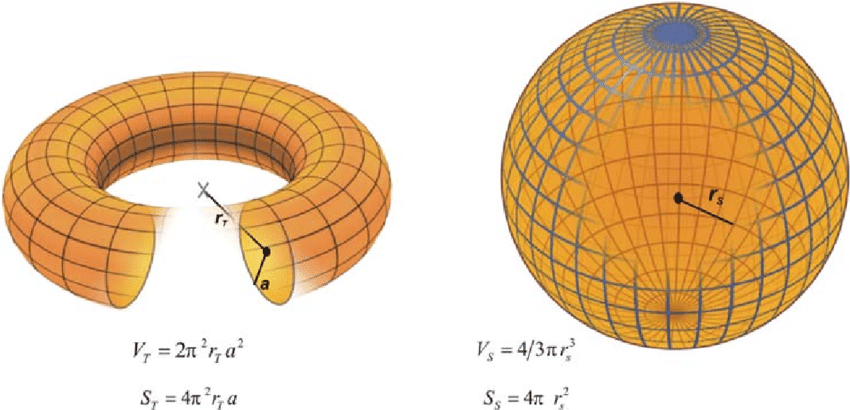
\includegraphics[width=\paperwidth,height=5cm]{title_fig.png}};
    \node[anchor=east] 
    at ([yshift=-35pt]current page.north east) (author)
    {\parbox[t]{.6\paperwidth}{\raggedleft%
            \usebeamerfont{author}\textcolor{black}{%
                \textpdfrender{
                    TextRenderingMode=FillStroke,
                        FillColor=black,
                        LineWidth=.1ex,
                }{\insertauthor}}}};
    \node[anchor=north east] 
    at ([yshift=-50pt]current page.north east) (institute)
    {\parbox[t]{.78\paperwidth}{\raggedleft%
            \usebeamerfont{institute}\textcolor{gray}{\insertinstitute}}};
    \node[anchor=south west] 
    at ([yshift=20pt]current page.west) (logo)
    {\parbox[t]{.19\paperwidth}{\raggedleft%
            \usebeamercolor[fg]{titlegraphic}\inserttitlegraphic}};
    \node[anchor=east]
    at ([yshift=-20pt]current page.north east) (title)
    {\parbox[t]{\textwidth}{\raggedleft%
            \usebeamerfont{author}\textcolor{purple}{%
                \textpdfrender{
                    TextRenderingMode=FillStroke,
                    FillColor=purple,
                    LineWidth=.1ex,
                }{\inserttitle}}}};
    \node[anchor=west]
    at ([yshift=-30pt]current page.north west) (subtitle)
    {\parbox[t]{.6\paperwidth}{\raggedleft\usebeamerfont{subtitle}\textcolor{black}{\insertsubtitle}}};
    \end{tikzpicture}
}
\begin{document}
    \begin{frame}[plain]
        \maketitle
    \end{frame}
\end{document}

% \begin{frame} \maketitle
% \end{frame}

\begin{frame}{T.O.C.: The Math}
  \tableofcontents[sections={1-3}]
\end{frame}

\begin{frame}{T.O.C.: Physical Systems}
  \tableofcontents[sections={4-6}]
\end{frame}


%-----------------------------THE IRRELEVANT PHASE-------------------------------------
\section{The Irrelevant Phase}
\begin{frame}{The Irrelevant Phase}
  
  \begin {enumerate}
    \item All quantum mechanical observables correspond to Hermitian operators 
          ($\hat{O}$).
    \item All Hermitian operators have a spectral decomposition
          ($\hat{O} = \sum_{n} a_{n} \ket{\Psi_{n}}\bra{\Psi_{n}}$).
        \item The projector components ($\ket{\Psi_{n}}\bra{\Psi_{n}}$) of the 
              spectrally decomposed operator $\hat{O}$ are all invariant under 
              the gauge transformation 
              $\ket{\Psi_{n}} \rightarrow \exp(i\alpha_{n}) \ket{\Psi_{n}}$.
  \end{enumerate}

  \vspace{2ex}

  $\Rightarrow$ Phase is not physical!
  \begin{align*}
    \Psi = \Psi \cdot exp(i\phi) && \phi \in \{0, \, 2\pi\}
  \end{align*}
  
\end{frame}

%----------------------------THE BERRY PHASE------------------------------------------
\section{The Berry Phase}

\subsection{The Discrete Case}
\begin{frame}{The Relative Phase}
 
  \begin{columns}
    \begin{column}{0.5\textwidth}


      \begin{itemize}
        \item The relative phase between two states can be uniquely defined for a given
              gauge.

        \item The relative phase is not invariant under local gauge transformations (i.e.
              multiplication of the state by a phase factor).   
      \end{itemize}

    \end{column}

    \begin{column}{0.5\textwidth}

      Relative Phase:
      \begin{equation*}
        \gamma_{1,2} = -arg \braket{\Psi_{1}|\Psi_{2}} \qquad \gamma_{1, 2} \in (-\pi, \pi]
      \end{equation*}

      Gauge Transformation:
      \begin{flalign*}
        &\ket{\Psi_{j}} \rightarrow \exp(i \alpha_{j}) \ket{\Psi_{j}}&\\ 
        &\exp(-i\gamma_{1,2}) \rightarrow \exp(-i\gamma_{1,2} + i(\alpha_{2} - \alpha_{1}))
      \end{flalign*}

    \end{column}
  \end{columns}

\end{frame}


\begin{frame}{The Berry Phase}

  \begin{columns}

    \begin{column}{0.5\textwidth}
  
      \begin{itemize}
        \item Summation of a non-gauge invariant quantity ($\gamma_{i,j}$) along closed loops
              results in a gauge-invariant result!
        \item The Berry Phase can be expressed in terms of gauge-invariant operators.
      \end{itemize}

    \end{column}

    \begin{column}{0.5\textwidth}
  
      The Berry Phase:
      \begin{equation*}
        \gamma_{L} = \sum_{i = 0}^{N-1} 
                     \gamma_{i \; \mathrm{mod} \; N, i+1 \; \mathrm{mod} \; N}
      \end{equation*}

      Invariance:
      \begin{equation*}
        \gamma_{L} = \Tr \left( 
                               \prod_{i = 0}^{N-1} \ket{\Psi_{i}} \bra{\Psi_{i}}
                         \right)
      \end{equation*}
    
    \end{column}
  \end{columns}
    
  \documentclass[tikz]{standalone}
\usepackage{tikz}
\usetikzlibrary{positioning}
\begin{document}
      \begin{tikzpicture}[                                                                     
                          bend angle=45,
                          roundnode/.style={                                                   
                                            circle,                                            
                                            draw=black!60,                                     
                                            fill=gray!5,                                       
                                            very thick,                                        
                                            minimum size=7mm                                   
                                           },
                         ]
        \node[roundnode] (top) at (90:1) {$\Psi_{4}$};
        \node[roundnode] (bottom) at (270:1) {$\Psi_{2}$};
        \node[roundnode] (left) at (180:1) {$\Psi_{1}$} 
          edge[<-, bend left] node[auto] {$\gamma_{4,1}$} (top)
          edge[->, bend right] node[auto, swap] {$\gamma_{1,2}$} (bottom); 
        \node[roundnode] (right) at (0:1) {$\Psi_{3}$}
          edge[->, bend right] node[auto, swap] {$\gamma_{3,4}$} (top)
          edge[<-, bend left] node[auto] {$\gamma_{2,3}$} (bottom); 
      \end{tikzpicture}
\end{document}


\end{frame}

\subsection{The Continuous Case}
\begin{frame}{By Analogy}
  
  \begin{columns}
    \begin{column}{0.5\textwidth}
      
      \textbf{Discrete}:
      \begin{itemize}
        \item<1-> Parameter Space: $\mathbb{P} = \mathbb{N}_{0}$
        \item<2-> Wave Function $\Psi: \mathbb{P} \rightarrow \mathcal{H}, \quad 
              n \mapsto \ket{\Psi_{n}}$
        \item<3-> Path: $\mathcal{C} = [n_{0}, n_{1}, \ldots, n_{N-1}]$
        \item<4-> Berry Phase: $\gamma(\mathcal{C}) = \sum_{i = 0}^{N} \gamma_{n_{i \; 
              \mathrm{mod} \; N}, n_{i+1 \; \mathrm{mod} \; N}}$\\

      \end{itemize}

      \vspace{3ex}
      \colorbox{lightgray}
      {
        \begin{minipage}{\textwidth}
          \onslide<5->{The sum of the relative phases of each wave function connected by the path 
          $\mathcal{C}$.}
        \end{minipage}
      }
    \end{column}
    \begin{column}{0.5\textwidth}
  
      \textbf{Continuous}:
      \begin{itemize}
        \item<1-> Parameter Space: $\mathbb{P} = \mathcal{M}$
        \item<2-> Wave Function $\Psi: \mathbb{P} \rightarrow \mathcal{H}, \quad \bm{R}
              \mapsto \ket{\Psi(\bm{R})}$
        \item<3-> Path: $\mathcal{C}: [0, 1) \rightarrow \mathcal{M}, \quad t \mapsto 
              \bm{R}(t)$
        \item<4-> Berry Phase: $\gamma(\mathcal{C}) = \lim_{dt \to 0} \oint
              \gamma_{\mathcal{C}(t), \mathcal{C}(t + dt)} d \bm{R}$
      \end{itemize}
      \vspace{3ex}
      \colorbox{lightgray}
      {
        \begin{minipage}{\textwidth}
          \onslide<5->{The integrated relative phase of all the wave functions connected by the path 
          $\mathcal{C}.$}
        \end{minipage}
      }
    \end{column}
  \end{columns}

\end{frame}

\begin{frame}{The Berry Connection}
  
  Relative Phase: 
  $\lim_{\bm{r} \to 0} \gamma_{\bm{R}, \bm{R} + \bm{r}} = \lim_{\bm{r} \to 0} 
  -arg \braket{\Psi(\bm{R}|\Psi(\bm{R} + \bm{r})}$  
  \vspace{2ex}
  \fbox{
    \begin{minipage}[t]{\textwidth}
      \begin{equation*}
        \begin{aligned}
          &\lim_{\bm{r} \to 0} \exp(-i \gamma_{\bm{R}, \bm{R + \bm{r}}}) = 
           \lim_{\bm{r} \to 0}\frac{\braket{\Psi(\bm{R})|\Psi(\bm{R} + \bm{r})}}
           {|\braket{\Psi(\bm{R})|\Psi(\bm{R} +\bm{r})}|}&\\
          &1 - i \gamma_{\bm{R}, \bm{R} + \bm{r}} = \bra{\Psi(\bm{R})}(\ket{\Psi(\bm{R})} 
                                               + \nabla_{\bm{R}} \ket{\Psi(\bm{R})})&\\
          &\Rightarrow \gamma_{\bm{R}, \bm{R + d\bm{r}}} =
           i\braket{\Psi(\bm{R})|\nabla_{\bm{R}}|\Psi(\bm{R})}
       \end{aligned}
     \end{equation*}
   \end{minipage}
  }

   \colorbox{lightgray}
   {
     \begin{minipage}{\textwidth}
       \begin{equation*}
         \gamma(\mathcal{C}) = \oint i \braket{\Psi(\bm{R})|\nabla_{\bm{R}}|\Psi(\bm{R})} d\bm{R}
       \end{equation*}
     \end{minipage}
   }

\end{frame}

\begin{frame}{The Berry Connection and Curvature}
  

       \begin{columns}[T]
    \begin{column}{0.5\textwidth}
       
      \begin{itemize}
        \item Discrete relative phase quantities in the discrete case are replaced by
              the Berry Connection in the continuous case.
        \item The Berry Connection is non-gauge invariant under gauge transformations.
      \end{itemize}


    \end{column}

    \begin{column}{0.5\textwidth}

       \begin{flalign*}
         &\textbf{Berry Connection:}&\\
         &\mathcal{A} := i \braket{\Psi(\bm{R})|\nabla|\Psi(\bm{R})}
       \end{flalign*}

       \begin{flalign*}
       &\textbf{Gauge Transformation:}&\\
       &\ket{\Psi(\bm{R})} \rightarrow \exp(i \alpha(\bm{R})) \ket{\Psi(\bm{R})}&\\
       & \mathcal{A} \rightarrow \mathcal{A} - \nabla \alpha(\bm{R})&\\
       \end{flalign*}

    \end{column}
  \end{columns}

\end{frame}

\begin{frame}{The Berry Connnection and Curvature}

  \begin{columns}
    \begin{column}{0.5\textwidth}

      \begin{itemize}
        \item Stokes' theorem can be utilized to reformulate the path integral to a
              surface integral.
      \end{itemize}

    \end{column}

    \begin{column}{0.5\textwidth}
       \begin{flalign*}
         &\textbf{Stokes' Theorem:}&\\
         &\gamma(\mathcal{C}) 
         = \sum_{\mu, \nu} \int_{\mathcal{S}(\mathcal{C})} 
         \frac{1}{2} \partial_{\mu} \mathcal{A}_{\nu} - \partial_{\nu} \mathcal{A}_{\mu} dR^{\mu}
         \wedge dR^{\nu}&
       \end{flalign*}
    \end{column}
  \end{columns}

\end{frame}

\begin{frame}{The Berry Connection and Curvature}

  \begin{columns}

    \begin{column}{0.5\textwidth}

      \begin{itemize}
        \item The resulting integrand defines what is known as the Berry Curvature.
        \item The Berry Curvature is gauge-invariant under gauge transformations.
      \end{itemize}

    \end{column}

    \begin{column}{0.5\textwidth}

       \begin{flalign*}
         &\textbf{Berry Curvature:}&\\
         &\Omega_{\mu, \nu}(\bm{R}) := \partial_{\mu} \mathcal{A}_{\nu} - \partial_{\nu} \mathcal{A}_{\mu}  
       \end{flalign*}

       \begin{flalign*}
         &\textbf{Gauge Transformation:}&\\
         &\ket{\Psi(\bm{R})} \rightarrow \exp(i\alpha(\bm{R}))\ket{\Psi(\bm{R})}&\\
         &\Omega_{\mu, \nu}(\bm{R}) \rightarrow \partial_{\mu} (\mathcal{A}_{\nu}
         - \partial_{\nu} \alpha(\bm{R})) - \partial_{\nu}(\mathcal{A}_{\mu} -
         \partial_{\mu} \alpha(\bm{R}))
      \end{flalign*}

    \end{column}

  \end{columns}

\end{frame}

\begin{frame}{Magnetic Analogies}

    \begin{itemize}
      \item The relationship between the Berry Phase ($\gamma$), Berry Connection
            ($\bm{\mathcal{A}}$) and Berry Curvature ($\bm{\Omega}$) is analogous to the 
            relationship between the magnetic flux ($\Phi$), magnetic vector potential
            ($\bm{A}$) and magnetic flux density ($\bm{B}$).
    \end{itemize}
  
  \begin{columns}
    
    \begin{column}{0.5\textwidth}

       \begin{align*}
         \textbf{Phase:}&\\
         \gamma(C) &= \oint \bm{\mathcal{A}} \cdot d\bm{R} \\
                   &= \int_{\mathcal{S}(\mathcal{C})} 
                      \nabla \times \bm{\mathcal{A}} \cdot d\bm{s}\\
                   &= \int_{\mathcal{S}(\mathcal{C})} \bm{\Omega} \cdot d\bm{s}
       \end{align*}
       
    \end{column}

    \begin{column}{0.5\textwidth}
    
      \begin{align*}
        \textbf{Flux:}&\\
        \Phi(C) &= \oint \bm{A} \cdot d\bm{R} \\
                &= \int_{\mathcal{S}(\mathcal{C})}
                   \nabla \times \bm{A} \cdot d\bm{s} \\
                &= \int_{\mathcal{S}(\mathcal{C})} \bm{B} \cdot d\bm{s}
      \end{align*}

    \end{column}
  \end{columns}

  
\end{frame}
           

%-------------------------------THE ADIABATIC THEOREM-----------------------------------
\section{The Adiabatic Theorem}

\subsection{Statement}
\begin{frame}{Statement}
  
  \begin{columns}[t]
    \begin{column}{0.6\textwidth}
  \begin{theorem}
    Under a slowly changing Hamiltonian with instantaneous eigenstates $\ket{n(t)}$ and
    energies $E_{n}(t)$, the state of a quantum system evolves 
    ($\Psi(t) = \sum_{n} c_{n}(t)\ket{n(t)}$) such that the amplitudes of the instantaneous
    eigenstates composing the wave function are given by:

    \begin{flalign*} 
        &c_{n}(t) = c_{n}(0)e^{i\theta_{n}(t)}e^{i\gamma_{n}(t)} &\\
        &\theta_{n}(t)  = -\hbar^{-1} \int_{0}^{t} E_{n}(t^{\prime}) dt^{\prime} &\\ 
        &\gamma_{n}(t) = i\int_{0}^{t} \braket{m(t^{\prime})|\dot{m}(t^{\prime})}
        dt^{\prime}
    \end{flalign*}

  \end{theorem}

    \end{column}
    \begin{column}{0.4\textwidth}
       
       \begin{flalign*}
         &\textbf{Assumptions}&\\
         &\text{\textbf{1.}} \quad i \hbar \ket{\dot{\Psi}(t)} 
         = \bm{H} \ket{\Psi(t)}&\\
         &\text{\textbf{2.}} \quad 
         \frac{\braket{m(t)|\dot{\bm{H}}(t)|n(t)}}{E_{m}(t) - E_{n}(t)} = 0 
       \end{flalign*}

    \end{column}
  \end{columns}

\end{frame}

\subsection{Proof}
\begin{frame}{Proof: Part I}
 
  \begin{columns}
    
    \begin{column}{0.4\textwidth}
      \begin{enumerate}
        \item Begin with the time-dependent Schrödinger equation.

        \item Expand $\ket{\Psi(t)}$ and apply the Hamiltonian $\bm{H}$ to the eigenstates
        $\ket{n(t)}$.

        \item Take the inner product of both sides of the equation with $\ket{m(t)}$.
      \end{enumerate}
    \end{column}

    \begin{column}{0.6\textwidth}
      
      \begin{flalign*}
        &i\hbar\ket{\dot{\Psi}(t)} = \bm{H}(t)\ket{\Psi(t)}&
      \end{flalign*}

      \begin{flalign*}
        & \bm{L.H.S} = \sum_{n} c_{n}(t) E_{n}(t) \ket{n(t)}&\\
        &i\hbar \sum_{n} \left[ \dot{c}_{n}(t)\ket{n(t)} + c_{n}(t)\ket{\dot{n}(t)}
        \right] = \bm{R.H.S}
      \end{flalign*}

      \begin{flalign*}
        &i\hbar \dot{c}_{m}(t) + i \hbar \sum_{n} \braket{m(t)|\dot{n}(t)}
        = c_{m}(t) E_{m}(t)&
      \end{flalign*}

    \end{column}
  \end{columns}
\end{frame}

\begin{frame}{Proof: Part II}
 
  \begin{columns}

    \begin{column}{0.4\textwidth}
      
      \begin{enumerate}
        \setcounter{enumi}{3}
        \item Differentiate the time-independent Schrödinger equation with respect to
              time.
        \item Take the inner product of both sides of the equation with $\ket{m(t)}$.
        \item Rearrange in terms of the inner product $\braket{m(t)|\dot{n}(t)}$.
      \end{enumerate}
    
    \end{column}

    \begin{column}{0.4\textwidth}
      
      \begin{flalign*}
        &\bm{L.H.S} = \dot{E}_{n}(t) \ket{n(t)} + E_{n}(t) \ket{\dot{n}(t)}&\\
        &\dot{\bm{H}}(t) \ket{n(t)} + \bm{H}(t) \ket{\dot{n}(t)} = \bm{R.H.S}
      \end{flalign*}

       \begin{flalign*}
         &\bm{L.H.S} =  E_{n}(t) \braket{m(t)|\dot{n}(t)}&\\
         &\braket{m(t)|\dot{\bm{H}}(t)|n(t)} + E_{m} \braket{m(t)|\dot{n}(t)} 
         = \bm{R.H.S} 
       \end{flalign*}
  
       \begin{flalign*}
         &\braket{m(t)|\dot{n}(t)} 
         = \frac{\braket{m(t)|\dot{\bm{H}}(t)|n(t)}}{E_{n}(t) 
         - E_{m}(t)} \quad (m \neq n)&
       \end{flalign*}

    \end{column}
  \end{columns}

\end{frame}

\begin{frame}{Proof: Conclusion}
  
  \begin{columns}
    \begin{column}{0.5\textwidth}

      \begin{enumerate}
        \setcounter{enumi}{6}
        \item Insert the result from Part II into the result from Part I.
        \item For $\braket{m(t)|\dot{\bm{H}}(t)|n(t)} \ll E_{m}(t) - E_{n}(t)$ and 
              $\forall n  \quad \forall t: E_{m}(t) - E_{n}(t) \neq 0$.
        \item Solving the resulting differential equation for $c_{m}(t)$.
      \end{enumerate}

    \end{column}
    
    \begin{column}{0.5\textwidth}

      \begin{flalign*}
        &\bm{L.H.S} = \sum_{\substack{n\\ n \neq m}} 
                      \frac{\braket{m(t)|\dot{\bm{H}}(t)|n(t)}}{E_{m}(t) - E_{n}(t)}&\\
        &\dot{c}_{m}(t) 
        + \left( \frac{i}{\hbar} E_{m}(t) + \braket{m(t)|\dot{m}(t)} \right)
        c_{m}(t) = \bm{R.H.S}
      \end{flalign*}

      \begin{flalign*}
        &\dot{c}_{m}(t)  
        = i \left( - \frac{1}{\hbar}E_{m}(t) + i\braket{m(t)|\dot{m}(t)} \right)
        c_{m}(t)&
      \end{flalign*}

      \begin{flalign*}
        &c_{m}(t) 
        = c_{m}(0) e^{-i \frac{1}{\hbar} \int_{0}^{t} E_{m}(t^{\prime}) dt^{\prime}}
        e^{i\int_{0}^{t} i\braket{m(t^{\prime})|\dot{m}(t^{\prime}}dt^{\prime}}&
      \end{flalign*}
    
    \end{column}
  \end{columns}

\end{frame}

\begin{frame}{Proof: The Berry Phase}
  
  Time evolution given by the variation of parameters $\bm{R} \in \mathbb{P}$:
  \begin{equation*}
    \bm{H}(t) = \bm{H}(\bm{R}(t)) \quad \Psi(t) = \Psi(\bm{R}(t))
  \end{equation*}

  Therefore:
  \begin{align*}
    \gamma &=  \int_{0}^{t} i \braket{m(\bm{R}(t))|\dot{m}(\bm{R}(t))} dt\\
           &=  \int_{0}^{t}
           i \braket{m(\bm{R}(t))|\nabla_{\bm{R}}|m(\bm{R}(t))} \dot{\bm{R}}(t) dt \\
           &= \oint i \braket{m(\bm{R})|\nabla_{\bm{R}}|m(\bm{R})}d\bm{R}
  \end{align*}
\end{frame}


%----------------------Magnetic Moment in a Precessing Field----------------------------
\section{Magnetic Moment in a Precessing Field}

\subsection{Defining the System}
\begin{frame}{Defining the System}
 
  \colorbox{lightgray}{
    \parbox{\textwidth}{
      \textbf{System}:\\ Magnetic moment at the origin in the presence of a magnetic field
                       $B$ of fixed magnitude, moving along some closed path 
                       $\mathcal{C}$.
    }
  }

      \begin{align*}
        \bm{B}(t) = B_{0} \begin{pmatrix} 
                                          \sin\theta(t)\cos\phi(t)\\
                                          \sin\theta(t)\sin\phi(t)\\
                                          \cos\theta(t)
                           \end{pmatrix}
        && \bm{H}(t) = \frac{\hbar e}{2m}\bm{B} \cdot \bm{\sigma}
      \end{align*}

  \begin{columns}

    \begin{column}{0.6\textwidth}


      \begin{align*}
        \chi_{+}(t) &= \begin{pmatrix} 
                                      \cos\frac{\theta(t)}{2}\\
                                      e^{i\phi(t)} \sin \frac{\theta(t)}{2}
                       \end{pmatrix} 
                       && E_{+} = \frac{\hbar \omega_{1}}{2}\\
       \chi_{-}(t) &= \begin{pmatrix} 
                                     e^{-i\phi(t)}\sin\frac{\theta(t)}{2}\\
                                     -\cos\frac{\theta(t)}{2}
                       \end{pmatrix} 
                       && E_{-} = -\frac{\hbar \omega_{1}}{2}
      \end{align*}
    \end{column}

    \begin{column}{0.4\textwidth}
      \begin{figure}
        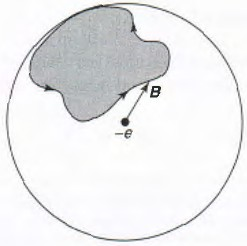
\includegraphics[width=0.8\textwidth]{b_spin_system_2}
      \end{figure}
    \end{column}
    
  \end{columns}

\end{frame}

\subsection{Calculating the Berry Phase}
\begin{frame}{Calculating the Berry Phase}

  \begin{columns}[t]

    \begin{column}{0.5\textwidth}
     
      The adiabatic approximation applies:
      \begin{flalign*}
        &\gamma = \int_{\mathcal{C}} i \braket{\chi_{+}|\nabla_{r, \theta, \phi}|\chi_{+}} \cdot
        d\bm{B}&\\
        &\braket{\chi_{+}|\nabla_{r, \theta, \phi}|\chi_{+}} = i \frac{\sin^{2}(\theta /
        2)}{r \sin(\theta)} \hat{\phi}
      \end{flalign*}


    \end{column}

    \begin{column}{0.5\textwidth}

      Applying Stokes' theorem:
      \begin{flalign*}
        &\gamma = \int_{\mathcal{S}(\mathcal{C})} i \nabla_{r, \theta, \phi} \times
        \braket{\chi_{+}|\nabla_{r, \theta, \phi}|\chi_{+}} \cdot d\bm{s}&\\
        &\nabla_{r, \theta, \phi} \times
        \braket{\chi_{+}|\nabla_{r, \theta, \phi}|\chi_{+}} = \frac{i}{2r^{2}}\hat{r}&\\
        &\gamma = -\frac{\Omega}{2}
      \end{flalign*}

    \end{column}

  \end{columns}

\end{frame}


%-----------------------------THE AHARANOV BOHM EFFECT----------------------------------
\section{The Aharonov-Bohm Effect}

\subsection{The Electric Effect}
\begin{frame}{The Electric Effect}

  \begin{enumerate}
    \item Electron beam is split at point A.
    \item Dual beams pass through \textit{Faraday Cages} to which a voltage is applied.
    \item Electron beams are recombined at point F.
  \end{enumerate}

  \vspace{2ex}

  \begin{minipage}{0.4\textwidth}
    \begin{flalign*}
      &\bm{H(t)} = \bm{H}_{0} + V(t) &\\
      &\Psi(t) = \Psi_{0} \exp(-i \mathcal{S}) &\\
      &\mathcal{S} = \int V(t) dt & 
    \end{flalign*}
  \end{minipage}
  \hspace{0.05\textwidth}
  \begin{minipage}{0.5\textwidth}
    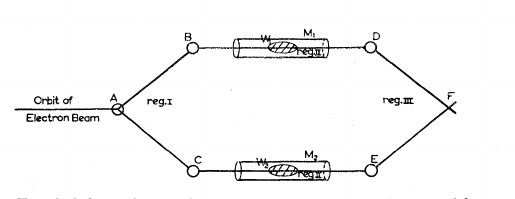
\includegraphics[width=\textwidth]{electric_effect}
    \captionof{figure}{Electric effect schematic.}
    \label{fig:ABE}
  \end{minipage}

\end{frame}

\subsection{The Magnetic Effect}
\begin{frame}{The Magnetic Effect}

  \begin{enumerate}
    \item Electron beam is split at point A.
    \item Dual beams pass over and under a solenoid coil producing a constant magnetic
      field in a infinitesimally small region at the origin.
    \item Electron beams are recombined at point F.
  \end{enumerate}

  \begin{minipage}{0.4\textwidth}
    \begin{align*}
      &\bm{H} = \frac{\left[ \bm{P} - \frac{e}{c}\bm{A} \right]^{2}}{2m} &\\
      &\Psi(t) = \Psi_{0} \exp(-i \mathcal{S}) &\\
      &\mathcal{S} = \int \bm{A} \cdot d\bm{x} &
    \end{align*}
  \end{minipage}
  \hspace{0.05\textwidth}
  \begin{minipage}{0.5\textwidth}
    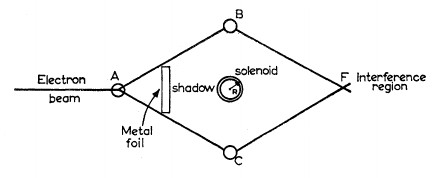
\includegraphics[width=\textwidth]{magnetic_effect}
    \captionof{figure}{Magnetic effect schematic.}
    \label{fig:AME}
  \end{minipage}

\end{frame}

\subsection{The Berry Phase}
\begin{frame}{The Berry Phase}
 
  \begin{columns}[t]
    \begin{column}{0.6\textwidth}

      The General Case:
      \begin{align*}
          &\bm{H} = \frac{\left[ \bm{P} - \frac{e}{c}\bm{A} \right]^{2}}{2m} + V(t) \\
          &\Psi(t) = \Psi_{0} \exp(-i \mathcal{S}) \\
          &\triangle \mathcal{S} = \oint V(t) dt + \bm{A} \cdot d\bm{x} 
      \end{align*}


    \end{column}

    \begin{column}{0.4\textwidth}

      The Berry Phase:
      \begin{equation*}
        \gamma = \oint i\braket{\Psi(t)|\nabla_{\bm{r}}|\Psi(t)} d\bm{r} = \mathcal{S}
      \end{equation*}

    \end{column}

  \end{columns}
\end{frame}

\section{Outlook}
% \begin{frame}{Outlook: Quantum Information Processing}

  % \begin{columns}
  %   \begin{column}{0.5 \textwidth}
      
      % \begin{itemize}
      %   \item Quantum information processing and the development of universal gates.
      %   \item Solid state physics and the classificatication of bands.
      %   \item Wavefront shaping of polarized light field fronts.
      %   \item Conductance in the quantum hall effect.
      % \end{itemize}

    % \end{column}

    % \begin{column}{0.5\textwidth}

       % \begin{figure}
       %   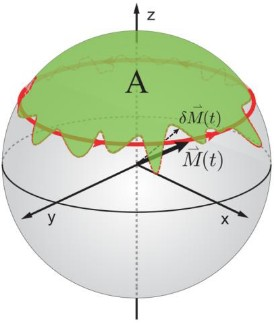
\includegraphics[width=0.5\textwidth]{geo_qbit}
       % \end{figure}
       % \begin{figure}
       %   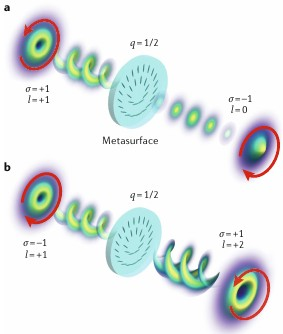
\includegraphics[width=0.5\textwidth]{wavefront}
       % \end{figure}

    % \end{column}
  % \end{columns}

% \end{frame}

\begin{frame}{Quantum Information}

  \begin{columns}
    \begin{column}{0.5 \textwidth}
      
      \begin{itemize}
        \item Use of the geometric phase in a universal set of quantum gates
        \item Fault tolerance because of geometric nature
      \end{itemize}

    \end{column}

    \begin{column}{0.5\textwidth}

       \begin{figure}
         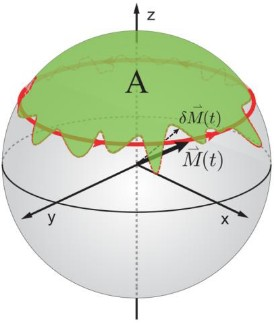
\includegraphics[width=0.5\textwidth]{geo_qbit}
       \end{figure}

    \end{column}
  \end{columns}

    \begin{align*}
      \hat{H} = \frac{1}{2}\begin{bmatrix}1 & 1 \\ 1 & -1\end{bmatrix}
      && \hat{\phi} = \begin{bmatrix} 1 & 0 \\ 0 & e^{i\phi}\end{bmatrix}
      && \hat{U}_{cphase} = \begin{bmatrix} 1 & 0 & 0 & 0 \\ 0 & 1 & 0 & 0 \\ 
                                        0 & 0 & 1 & 0 \\ 0 & 0 & 0 & e^{i\phi}
                        \end{bmatrix}
   \end{align*}

\end{frame}

\begin{frame}{Quantum Hall Effect}
  
  \begin{columns}

    \begin{column}{0.5\textwidth}
      \begin{itemize}
        \item Quantized conductivity closely related to the Berry curvature
          ($\Omega_{n}$) in the Thoules, Kohomoto, Nightingale and den Nijs (TKNN) formalism.
      \end{itemize}

      \begin{equation*}
        \sigma_{xy} = \frac{e^{2}}{\hbar} \sum_{n} \int \frac{dk}{2\pi} \Omega_{z}^{n}
      \end{equation*}

    \end{column}

    \begin{column}{0.5\textwidth}
      \begin{figure}
        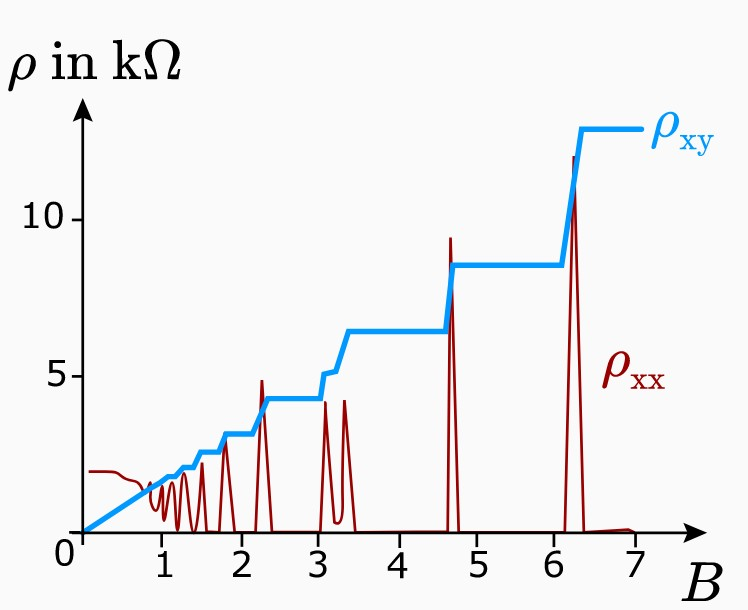
\includegraphics[width=0.7\textwidth]{quantum_hall}
      \end{figure}
    \end{column}
  \end{columns}

\end{frame}

\begin{frame}{Conclusion}
  
  \centering
  \colorbox{lightgray}
  {
    \begin{minipage}{0.8\textwidth}
    \begin{itemize}
      \item The Berry Phase is a gauge-invariant property of the manifold describing
            the parameter space of the system.
      \pause
      \item It is given as the integral of the berry connection over the parametrized
        path ($\oint i \braket{\Psi(\bm{R})|\nabla|\Psi(\bm{R})}$) which can be
        considered as the relative phase of two infinitesimally close states.
      \pause
      \item The Berry Phase arises naturally in the adiabatic theorem describing the
            quantum evolution of a state in a system undergoing infinitesimally small changes
            to its parameters.
      \pause
      \item The Berry Phase is just one example of the much wider phenomena of holonomy.
    \end{itemize}
  \end{minipage}
  }

\end{frame}

\end{document}
